\documentclass[a4paper,12pt]{article} % добавить leqno в [] для нумерации слева
\usepackage[a4paper,top=1.3cm,bottom=2cm,left=1.5cm,right=1.5cm,marginparwidth=0.75cm]{geometry}
%%% Работа с русским языком
\usepackage{cmap}					% поиск в PDF
\usepackage{mathtext} 				% русские буквы в фомулах
\usepackage[T2A]{fontenc}			% кодировка
\usepackage[utf8]{inputenc}			% кодировка исходного текста
\usepackage[english,russian]{babel}	% локализация и переносы

\usepackage{graphicx}

\usepackage{wrapfig}
\usepackage{tabularx}

\usepackage{hyperref}
\usepackage[rgb]{xcolor}
\hypersetup{
colorlinks=true,urlcolor=blue
}
\usepackage{multirow}
\usepackage{hhline}


%%% Дополнительная работа с математикой
\usepackage{amsmath,amsfonts,amssymb,amsthm,mathtools} % AMS
\usepackage{icomma} % "Умная" запятая: $0,2$ --- число, $0, 2$ --- перечисление

%% Номера формул
\mathtoolsset{showonlyrefs=true} % Показывать номера только у тех формул, на которые есть \eqref{} в тексте.

%% Шрифты
\usepackage{euscript}	 % Шрифт Евклид
\usepackage{mathrsfs} % Красивый матшрифт

%% Свои команды
\DeclareMathOperator{\sgn}{\mathop{sgn}}

%% Перенос знаков в формулах (по Львовскому)
\newcommand*{\hm}[1]{#1\nobreak\discretionary{}
{\hbox{$\mathsurround=0pt #1$}}{}}

\begin{document}
	
	\begin{titlepage}
	\begin{center}
		{\large МОСКОВСКИЙ ФИЗИКО-ТЕХНИЧЕСКИЙ ИНСТИТУТ (НАЦИОНАЛЬНЫЙ ИССЛЕДОВАТЕЛЬСКИЙ УНИВЕРСИТЕТ)}
	\end{center}
	\begin{center}
		{\large Физтех-школа электроники, фотоники и молекулярной физики}
	\end{center}
	
	
	\vspace{4.5cm}
	{\huge
		\begin{center}
			{Реферат}\\
			Графеновые транзисторы
		\end{center}
	}
	\vspace{2cm}
	\begin{flushright}
		{\LARGE Салтыкова Дарья \\
			\vspace{0.5cm}
			Б04-105}
	\end{flushright}
	\vspace{8cm}
	\begin{center}
		Долгопрудный 2022
	\end{center}
\end{titlepage}


\newpage

\section{Введение}
\noindent Графен — это углеродная пленка толщиной в один атом. Ее называют двумерной, потому что, в отличие от обычного трехмерного кристалла, положение каждого ее узла описывается не тремя, а только двумя координатами. Благодаря своей двумерности графен обладает целым рядом совершенно уникальных физических свойств, которые делают его перспективным материалом для электроники.
\medskip
\noindent У атомов углерода четыре орбитали на внешнем энергетическом уровне заполнены и еще четыре вакантны, поэтому они необычайно активны. Они легко вступают в соединения друг с другом, образуя разнообразные пространственные структуры: алмазы, графиты, графен, нанотрубки и фуллерены.
\medskip
\noindent Есть мнение, что графен может сильно изменить жизнь человека в XXI веке. Это не только самый тонкий материал, он также примерно в 200 раз прочнее стали и проводит электричество при комнатной температуре лучше, чем любой другой материал, известный человечеству.
\medskip
\noindent Электроны в графене в некоторых отношениях ведут себя так, словно у них вовсе нет массы. Это делает их похожими на безмассовые фотоны и позволяет использовать графен как лабораторию по исследованию релятивистских эффектов в квантовой механике. Причем роль скорости света тут играет особая скорость Ферми, которая примерно в 300 раз меньше скорости света. А если еще учесть, что в природе не существует безмассовых заряженных частиц, то электроны в графене представляют собой совершенно уникальную физическую систему.
\medskip
\noindent Парадокс Клейна состоит в том, что релятивистской, то есть движущейся с околосветовой скоростью, частице легче преодолеть высокий потенциальный барьер (превышающий две ее массы покоя), чем низкий. Это обеспечивает очень высокую подвижность электронов в графене.
\medskip
\noindent Самая захватывающая перспектива графена — это перевод на его основу всей микроэлектроники. У самых передовых полупроводниковых фирм в ходу 19-нанометровая технология. Это значит, что элементы имеют поперечник в две-три сотни атомов и уже близок предел миниатюризации кремниевых устройств. К тому же с повышением рабочей частоты электроника начинает сильно греться и дальнейшей миниатюризации мешают трудности теплоотвода. Благодаря нулевой эффективной массе электронов графена удается создавать чрезвычайно быстродействующие устройства. На сегодня в экспериментах уже достигнута частота свыше 100 ГГц. Высокая подвижность электронов в графене обеспечивает и высокую теплопроводность. 
\section{Свойства графена}
\begin{figure}[h!]
\center{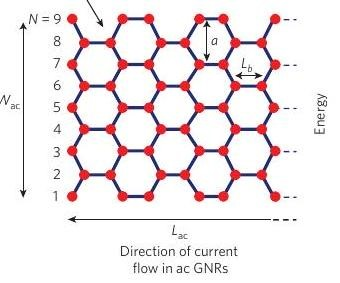
\includegraphics[scale={1.2}]{решетка.jpg}}
\caption{Схема кристаллической решетки графена}
\end{figure}
\noindent Кристаллическая решётка графена представляет собой плоскость, состоящую из шестиугольных ячеек, то есть является двумерной гексагональной кристаллической решёткой. Расстояние между ближайшими атомами углерода в шестиугольниках составляет 0,142 нм.
\medskip
\noindent Самым интересным свойством графена (так же как и ультратонкого графита), которое удалось обнаружить на данный момент, которое отличает его от других аллотропных модификаций углерода и дающим ему большие перспективы применения в электронике, является возможность управлять проводимостью тонких пленок с помощью внешнего электрического поля. Исследования показали, что при таком воздействии данные материалы стабильны, в отличие от других модификаций углерода.
\medskip
\noindent Так как графен является полуметаллом с нулевой шириной запрещенной зоны, то под действием электрического поля можно изменять концентрацию носителей зарядов. Экспериментально это делается следующим образом. Графеновый листок находится на кремниевой подложке, покрытой диэлектрическим слоем из $SiO^{2}$. Достаточно сильно легированный кремний можно использовать в качестве обратного затвора. При приложении к нему положительного напряжения в графене увеличивается концентрация свободных электронов, а при отрицательном – дырок. Концентрация носителей тока может достигать величины 1013 $\text{см}^{-2}$. Во всем диапазоне этих концентраций сохраняется высокая подвижность электронов и дырок вплоть до 2*104 $\text{см}^{2}\text{В}^{-1}\text{с}^{-1}$.
\medskip
\noindent Впервые именно у графена удалось наблюдать эффект Холла при комнатной температуре благодаря высокой подвижности носителей. Так же, он является природным двумерным газом.
\section{Туннельный полевой транзистор из графеновой гетероструктуры}
\noindent Графеновый полевой транзистор — транзистор из графена, который использует электрическое поле, создаваемое затвором для управления проводимостью канала. На сегодняшний момент не существует промышленного способа получения графена, но предполагается, что его хорошая проводимость поможет создать транзисторы с высокой подвижностью носителей и по этому показателю превзойти подвижность в полевых транзисторах на основе кремниевой технологии.
\medskip
\noindent Из-за отсутствия в графене запрещенной энергетической зоны отношение токов $\frac{I_{on}}{I_{off}}$ в открытом и закрытом состояниях транзисторов на основе графена очень мало и не превышает 10 при комнатной температуре. Этого достаточно для высокочастотных устройств и аналоговой электроники, но для цифровых (логических) интегральных схем такие транзисторы не годятся. Чтобы индуцировать в графене диэлектрическую щель, предлагалось использовать двухслойный графен, графеновые наноленты, различные химические модификации графена и пр. Однако особых успехов на этом пути достигнуто не было, поскольку ширина запрещенной зоны получалась слишком малой. В очередной работе группы Новоселова-Гейма предложен альтернативный вариант графенового полевого транзистора, работа которого основана на квантовом туннелировании электронов из графенового электрода через тонкий (~ 1 нм) слой гексагонального нитрида бора. Специфический линейный закон дисперсии электронов в графене приводит к тому, что плотность электронных состояний вблизи дираковской точки оказывается очень низкой, и поэтому при подаче на затвор напряжения $\V_g$, энергия Ферми в графеновом электроде $\Gr_B$ увеличивается гораздо быстрее, чем в обычном двумерном электронном газе с квадратичной дисперсией.
\begin{figure}[h!]
\center{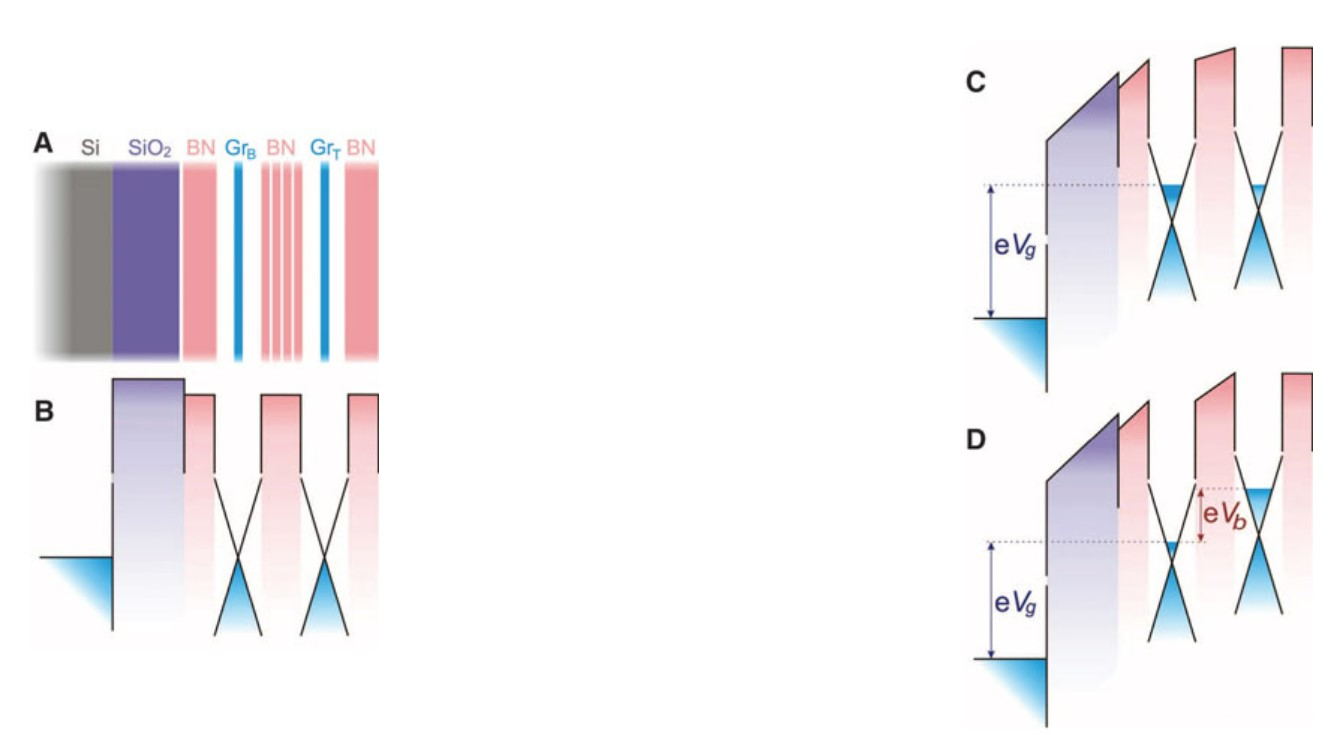
\includegraphics[scale={0.7}]{первая.jpg}}
\caption{(А) Схематическое изображение полевого транзистора
 с графеновыми электродами и затвором из гексагонального нитрида бора.
(B-D) Зонная структура в отсутствие напряжения на затворе;
при конечном напряжении на затворе и нулевом напряжении смещения;
при конечных значениях напряжения на затворе и напряжения смещения.}
\end{figure}
\noindent Графен является бесщелевым полупроводником с линейной зависимостью энергии квазичастиц $\epsilon$ от квазиимпульса p в окрестности экстремумов энергетической зоны:
$$\epsilon = \pm v_F p$$
\noindent где $vF = 106$ м/с — характерная скорость электронов в графене, знаки плюс и минус относятся соответственно к зоне проводимости и валентной зоне. Именно отсутствие запрещенной зоны в однослойном графене и малая (порядка 0.1 эВ) величина запрещенной зоны в двухслойном графене, узких полосках графена и полупроводниковых нанотрубках приводят к малому отношению токов открытого и закрытого состояний в полевых транзисторах на их основе. Одним из возможных решений проблемы является добавление туннельного контакта в канал транзистора. При этом проводимость канала может изменяться при варьировании напряжения на затворе по двум причинам: во-первых, благодаря изменению прозрачности туннельного барьера, во-вторых, благодаря изменению энергии Ферми в графене, ведущей к изменению плотности состояний туннелирующих электронов. Впервые была предложена следующая конструкция туннельного транзистора на основе графена: вертикальная конструкция представляла собой два параллельных листа графена (сток и исток), разделенных туннельно прозрачной диэлектрической прослойкой из нитрида бора. И высота туннельного барьера, и концентрация электронов в контактах регулировались нижним затвором. Влияние затвора на проводимость канала в данном устройстве, как показали измеренные характеристики, было слабым (неэкспоненциальным), и отношение токов открытого и закрытого состояния достигало лишь 50. Рассмотрим еще одну конструкцию туннельного полевого транзистора на основе графена. Зависимость тока от напряжения на затворе в предлагаемой структуре является экспоненциальной, а обратная крутизна подпороговой характеристики приближается к $(60 \text{мВ/дек}) \^{−1}$ при комнатной температуре.
\section{Конструкция прибора}
\noindent Туннельный контакт в предлагаемых вариантах транзистора представляет собой контакт листа графена с диэлектриком (полупроводником). Для обеспечения большого тока открытого состояния туннельная прозрачность барьера должна быть достаточно высокой, а значит, барьер должен быть либо узким, либо низким (т. е. работа выхода из графена в материал туннельного контакта должна быть небольшой). Высота барьера определяется материалом туннельного контакта, она сравнительно высока для диэлектрических материалов. На границе ”графен–гексагональный нитрид бора“ эта высота составляет 1.5 эВ для дырок и 4 эВ для электронов. Для уменьшения работы выхода в качестве туннельного контакта можно использовать полупроводниковый материал (например, кремний). В этом случае высота барьера приблизительно равна половине ширины запрещенной зоны полупроводника. Две предлагаемые конструкции туннельных полевых транзисторов с графеновыми каналами схематически изображены на рис. в поперечном разрезе. На рис. a кремниевая вставка шириной L помещена в центр проводящего канала, а лист графена окружен диэлектриком. Для обеспечения высокой подвижности и малого наведенного заряда в канале может быть использован гексагональный нитрид бора. Проводимость канала управляется верхним затвором, находящимся на расстоянии d от листа графена. На рис. b кремниевый туннельный контакт расположен около стока, причем контакты стока и затвора разделены диэлектрическим спейсером, который может быть сформирован, например, при окислении металлического электрода. Структура может управляться как верхним, так и нижним затвором.
\begin{figure}[h!]
\center{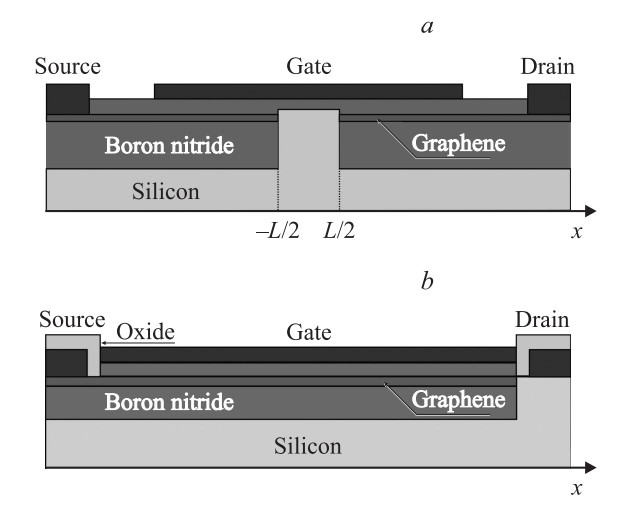
\includegraphics[scale={1}]{1.jpg}}
\caption{ Схематическое изображение предлагаемых транзисторных структур: a — туннельный контакт внутри канала; b — туннельный контакт у стока.}
\end{figure}
\section{Зонные диаграммы и распределение потенциала в канале транзистора}
\noindent Для расчета характеристик предполагаемого транзистора необходимо знать распределение локального электрического потенциала в канале транзистора $\phi$ как функцию напряжения на затворе $V_G$ и туннельную прозрачность барьера d. Вдали от туннельного контакта и электродов стока и истока локальный потенциал в канале (по отношению к заземленному истоку) не зависит от координаты и равен $\phi_0$. Это значение может быть найдено из модели плоского конденсатора, дающей локальную связь плотности заряда и напряжения:
$$ \frac{kk_0}{d} (V_G-\phi_0) = e[n_e(\phi_0)-n_h(\phi_0)]$$
\noindent где $k$ — диэлектрическая проницаемость подзатворного диэлектрика (k = 5.04 для гексагонального нитрида бора), $k_0$ — электрическая постоянная, e > 0 — элементарный заряд, $n_e$ и $n_h$ — концентрации электронов и дырок, рассчитанные на единицу площади. Предполагая, что уровень Ферми в графене у контактов истока и стока расположен точно между зоной проводимости и валентной зоной (т. е. в так называемой дираковской точке), можно рассчитать концентрации электронов и дырок в канале. Так как $e\phi_0$ есть локальная энергия Ферми, при низких температурах (kT $\ll eϕ_0$) и положительном потенциале затвора для концентрации электронов получается следующее простое выражение:
$$n_e = \frac{e^2 {\phi_0}^2}{\pi \hbar^2 {v_F}^2}$$
\noindent Соответственно локальный потенциал в канале дается выражением
\begin{figure}[h!]
\center{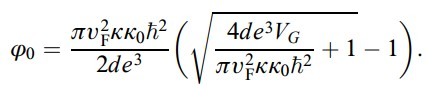
\includegraphics[scale={1}]{ф4.jpg}}
\end{figure}
\noindent Потенциал в туннельном контакте, определяющий высоту барьера для туннелирующих электронов, для структур с барьером в центре канала существенно зависит от отношения L/d. Разумно предположить, что для длинных барьеров при L $\dd$ d потенциал внутри барьера равен $V_G$ почти везде, кроме области вблизи границ. При L $\ll$ d потенциал затвора, наоборот, практически не ”проникает“ в туннельный зазор. В этом случае высота барьера (отсчитанная от дираковской точки) не зависит от напряжения на затворе, и роль последнего сводится к регулированию концентрации носителей заряда в графене. Аналогичная ситуация имеет место на рис. b, где туннельный контакт расположен вне подзатворной области и потенциал затвора практически не влияет на высоту барьера. В дальнейшем мы рассмотрим два характерных профиля потенциала вдоль канала транзистора. Первый соответствует относительно длинным туннельным зазорам в центре канала (как на рис. a), соответствующая зонная диаграмма представлена на рис. Второй тип распределения соответствует транзистору с туннельным контактом вне подзатворной области (как на рис. b), соответствующая зонная диаграмма представлена на рис. Предположим также, что приложенное между стоком и истоком напряжение целиком падает на туннельном контакте. Это оправдано, если сопротивление туннельного контакта превышает сопротивление листа графена. В обоих случаях туннельный барьер будет считаться трапециевидным.
\begin{figure}[h!]
\center{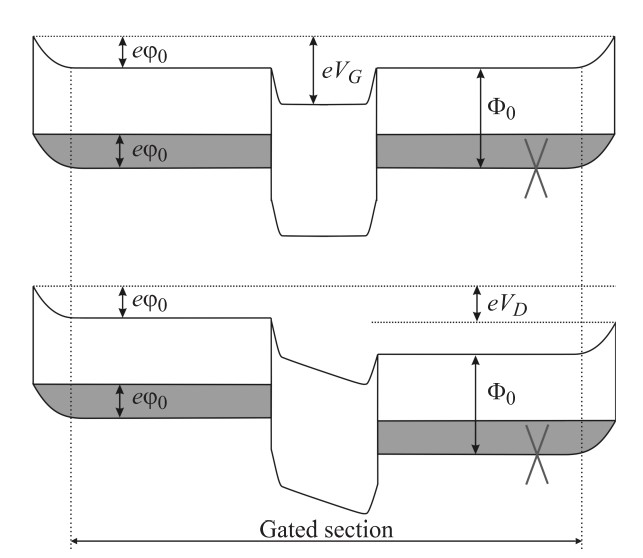
\includegraphics[scale={1}]{2.jpg}}
\caption{ Зонные диаграммы для транзистора на основе графена с туннельным контактом внутри канала (L $\dd$ d) при нулевом напряжении на стоке (сверху) и при положительном напряжении на стоке $V_D$ . Положение дираковской точки показано крестом.}
\end{figure}

\begin{figure}[h!]
\center{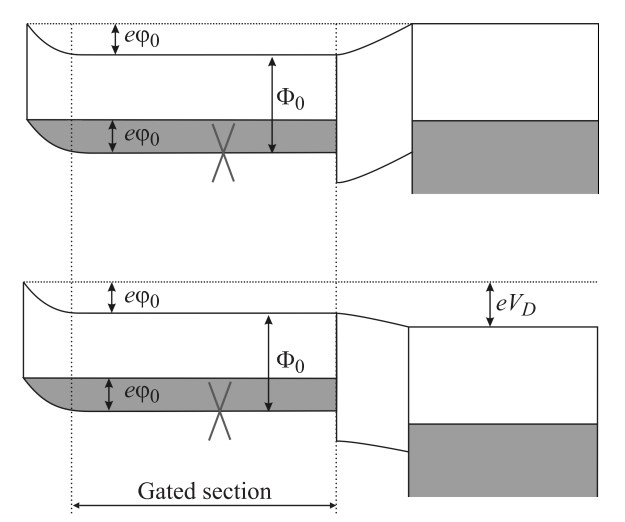
\includegraphics[scale={1}]{3.jpg}}
\caption{ Зонные диаграммы для транзистора на основе графена с туннельным контактом около стока при нулевом напряжении на стоке (сверху) и при положительном напряжении на стоке $V_D$. Положение дираковской точки показано крестом.}
\end{figure}

\section{Расчет туннельного тока}
\noindent Туннелирование через запрещенную зону полупроводников изучалось в работах Кейна и Келдыша в середине прошлого века, однако обобщение этих работ, учитывающее точную зонную структуру кремния, появилось сравнительно недавно. Теоретическая модель туннелирования через запрещенную зону в системе ”графен–кремний“ еще не разработана, и она заслуживает отдельного исследования. В дальнейших расчетах мы применим упрощенную модель, достаточную для предварительных оценок характеристик транзистора. Модель основана на квазиклассическом описании туннелирования:
\begin{figure}[h!]
\center{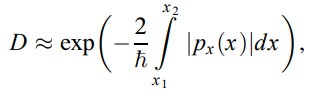
\includegraphics[scale={1}]{ф5.jpg}}
\end{figure}
\noindent где x1 и x2 — классические точки поворота, а проекция импульса $p_x$ в области барьера может быть найдена из условия сохранения энергии и поперечной (к оси x) компоненты импульса:
\begin{figure}[h!]
\center{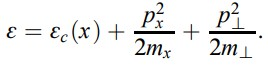
\includegraphics[scale={1}]{ф6.jpg}}
\end{figure}
\noindent В данном выражении εc (x) есть энергия дна зоны проводимости в туннельном контакте, mx — эффективная масса туннелирования, которая фактически является подгоночным параметром при сравнении теоретических расчетов с экспериментальными измерениями, и m⊥ — поперечная эффективная масса; вообще говоря, указанные массы могут быть разными. Вычисление прозрачности для трапециевидного барьера дает следующий результат:
\begin{figure}[h!]
\center{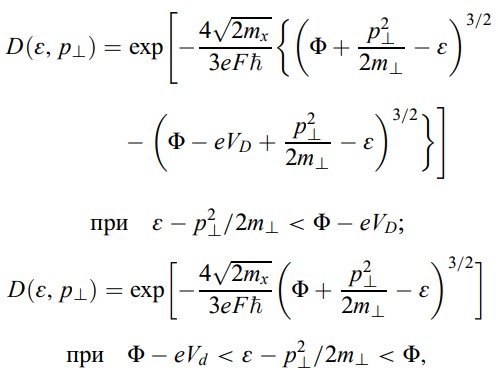
\includegraphics[scale={1}]{ф7.jpg}}
\end{figure}
\noindent где 8 — эффективная высота барьера для структур с длинным туннельным зазором (L $\dd$ d) в центре канала (рис. a). Она эффективно управляется напряжением на затворе:
$$ \text{Ф}_A = \text{Ф}_0 + e(\phi_0 – V_G) $$
\noindent В структурах же с коротким туннельным зазором около стока (рис. b, зонная диаграмма на рис.) эффективная высота барьера от напряжения на затворе не зависит. В данных выражениях есть работа выхода из графена в материал туннельного контакта при нулевом напряжении на затворе, отсчитанная от дираковской точки в графене. Величина F в уравнении означает напряженность поля в зазоре. Выражения для этой величины различны для двух предлагаемых структур (соответственно для структуры на рис. a и b):
\begin{figure}[h!]
\center{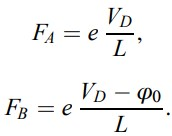
\includegraphics[scale={1}]{ф9-10.jpg}}
\end{figure}
\noindent Авторы работы предложили использовать в качестве mx ”легкую“ массу зоны проводимости, так как туннельная прозрачность барьера для легких носителей наибольшая, и соответственно они дают основной вклад в ток. В дальнейших вычислениях мы используем следующие параметры зонной структуры: $m_x$ = 0.19$m_e$, $m_t$ = 0.98$m_e$ , где $m_e$ — масса свободного электрона, 80 = 1/2 = 0.56 эВ, где 1 = 1.12 эВ — ширина запрещенной зоны в кремнии. Зная распределение потенциала и туннельную прозрачность барьера, мы можем применить известную ”баллистическую“ формулу для расчета тока туннельного транзистора. Для уменьшения количества уравнений в промежуточных расчетах мы не будем отдельно рассматривать туннельный и термоэмиссионный токи и положим прозрачность туннельного барьера равной единице при ε − p 2 ⊥/2m⊥ > 8. В данных обозначениях выражение для плотности тока между стоком и истоком принимает вид
\begin{figure}[h!]
\center{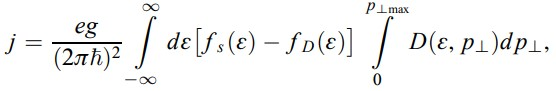
\includegraphics[scale={1}]{ф11.jpg}}
\end{figure}
\noindent где g = 4 — электронный фактор вырождения в графене, f S и f D — функции распределения Ферми в контактах истока и стока соответственно. Если начало отсчета энергии расположено в дираковской точке, то эти функции имеют вид
\begin{figure}[h!]
\center{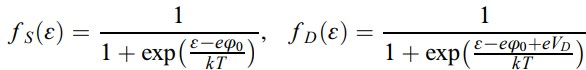
\includegraphics[scale={0.7}]{ф12.jpg}}
\end{figure}
\noindent Интегрирование по поперечной компоненте импульса проводится от нуля до максимального значения при заданной энергии $p⊥max = ε/v_F$, а интегрирование по энергии может быть распространено на весь интервал $(-\inf, +\inf)$, так как функция Ферми (при больших энергиях) и прозрачность барьера (при малых энергиях) спадают экспоненциально быстро. Следует отметить, что состояния с отрицательными энергиями заняты электронами валентной зоны графена, которые также могут давать вклад в туннельный ток.
\section{Обсуждение результатов}
\noindent Рассчитанные зависимости тока транзистора, включающего туннельную и термоэмиссионную компоненты, от напряжений на стоке и затворе представлены на рис. 4−7 для двух типов предложенных структур. Еще не проводя вычислений, можно предположить, что транзистор с длинным туннельным зазором в центре канала будет эффективнее управляться затвором по сравнению с транзистором с зазором у стока. Действительно, плотность тока в транзисторе с туннельным контактом в центре канала спадает экспоненциально при напряжениях на затворе, меньших работы выхода из графена в полупроводник (eVG < 80). Подпороговая крутизна характеристики, рассчитанная при d = 1 нм и L = 5 нм (рис. 4), равна kT/e, что говорит о преобладании термоэмиссионной компоненты тока над туннельной. Такое соотношение между двумя компонентами тока характерно также для туннельных транзисторов с контактом Шоттки и высокой прозрачностью туннельного барьера, на что было указано в работе. В отличие от классических кремниевых МОП транзисторов на объемной подложке, изменение проводимости в предлагаемой структуре обусловлено не только снижением высоты барьера, но и изменением энергии Ферми $e\phi_0$ в графеновых контактах. Последний эффект особенно важен в случае тонких диэлектриков. Подстановка значений $V_G$ = 2 В, d = 1 нм и κ = 5.06 в уравнение (4) дает энергию Ферми в контакте стока, равную 0.7 эВ, что превышает высоту барьера на границе раздела графен–кремний. Говоря образно, при столь высоких напряжениях на затворе электроны могут беспрепятственно ” выливаться“ из истока в сток. Зависимости тока транзистора от напряжения на стоке, выходящие на насыщение (см. рис.), схожи с аналогичными зависимостями для классических МОП транзисторов на объемной подложке. Слабая зависимость тока насыщения от напряжения на стоке обусловлена именно туннельным током, так как увеличение напряжения на стоке приводит к увеличению напряженности поля в зазоре и, следовательно, к увеличению прозрачности барьера. Ток включенного состояния предлагаемого транзистора довольно высок по сравнению с током кремниевых транзисторов, что является следствием высокой инжекционной способности графенового контакта. Кремниевая вставка в канале не ограничивает максимальный ток транзистора, так как движение электрона в туннельном кремниевом контакте при L = 5 нм является баллистическим. Характеристики туннельного транзистора на графене с коротким туннельным зазором вблизи стока ведут себя совершенно иным образом. Некоторые особенности характеристик, такие как неэкспоненциальное убывание тока при малых напряжениях на затворе, отсутствие насыщения, схожи с представленными в работе для транзистора с вертикальным туннелированием. Ранее уже было упомянуто, что степенная зависимость тока от напряжения на затворе наблюдается, если затвор влияет только на плотность состояний туннелирующих электронов, но не на высоту барьера. В двумерных системах с линейным спектром туннельная плотность состояний пропорциональна энергии Ферми $e\phi_0$, которая в свою очередь зависит квадратично от напряжения на затворе. В структурах с коротким туннельным зазором (L = 1 нм, d = 5 нм для характеристик на рис. 6 и 7) основная компонента тока — туннельная, и поэтому высокие токи включенного состояния, предсказанные для предыдущей конструкции, здесь недостижимы. Несмотря на то, что основная доля тока в структурах с коротким туннельным зазором обусловлена туннелированием, подпороговая крутизна характеристики данного транзистора по-прежнему ограничена термоэмиссионным пределом kT/e. Известно, что крутизна зависимости туннельного тока от напряжения на затворе может принимать любое значение. Однако при высокой крутизне туннельного тока сам туннельный ток мал (по сравнению с термоэмиссионным), и наоборот. Более строгое доказательство, касающееся ограничения крутизны данного транзистора (а также любого транзистора с барьером Шоттки), приведено в Приложении. Полученные значения плотности тока являются лишь грубыми оценками. Существует несколько неучтенных факторов, которые могут изменить эту оценку в лучшую или в худшую сторону. Во-первых, пространственный заряд в туннельном зазоре может ограничить рост тока при высоких напряжениях на затворе. Во-вторых, отражение электронов на границе раздела графен-кремний может значительно уменьшить значение прозрачности барьера. В-третьих, локальное значение энергии Ферми в графене в непосредственной близости от туннельного контакта превосходит $e\phi_0$. Этот факт, опущенный в предыдущих вычислениях, напротив, приведет к более высокой оценке плотности тока.

\begin{figure}[h!]
\center{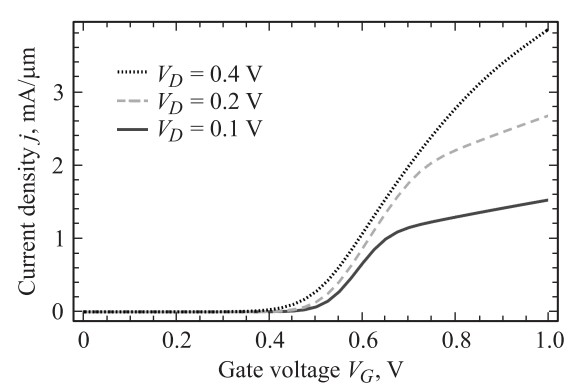
\includegraphics[scale={1.1}]{1график.jpg}}
\caption{ Зависимости плотности тока от напряжения на затворе для транзистора с туннельным контактом в центре канала. Ширина барьера L = 5 нм, толщина подзатворного диэлектрика d = 1 нм, температура T = 300 К.}
\end{figure}

\begin{figure}[h!]
\center{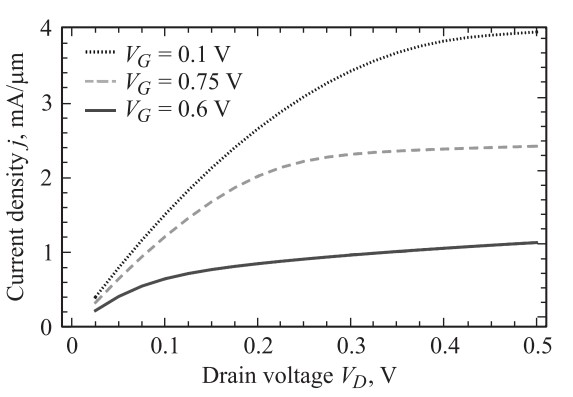
\includegraphics[scale={1.1}]{2график.jpg}}
\caption{ Зависимости плотности тока от напряжения на стоке для транзистора с туннельным контактом в центре канала. Ширина барьера L = 5 нм, толщина подзатворного диэлектрика d = 1 нм, температура T = 300 K.}
\end{figure}

\begin{figure}[h!]
\center{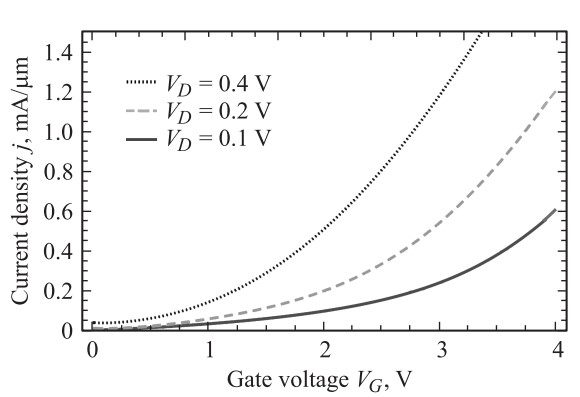
\includegraphics[scale={1.1}]{3график.jpg}}
\caption{ . Зависимости плотности тока от напряжения на затворе для транзистора с туннельным контактом около стока. Ширина барьера L = 1 нм, толщина подзатворного диэлектрика d = 5 нм, температура T = 300 K.}
\end{figure}

\begin{figure}[h!]
\center{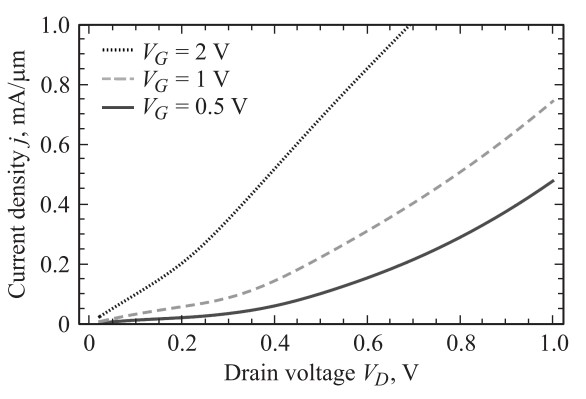
\includegraphics[scale={1.1}]{4график.jpg}}
\caption{ Зависимости плотности тока от напряжения на стоке для транзистора с туннельным контактом около стока. Ширина барьера L = 1 нм, толщина подзатворного диэлектрика d = 5 нм, температура T = 300 K.}
\end{figure}



\newpage

\section{Список использованной литературы}

\noindent Д.А. Свинцов, В.В. Вьюрков, В.Ф. Лукичёв, А.А. Орликовский, А. Буренков , Р. Охснер - Туннельные полевые транзисторы на основе графена. Физико-технологический институт Российской академии наук, 117218 Москва, Россия; Институт интегральных схем общества Фраунгофера, 91058 Эрланген, Германия.

\medskip

\noindent Schwierz, F. \& Liou, J. J. Modern Microwave Transistors - Theory, Design, and by copper and is comparable with those supported by nanotubes) ${ }^{95}$ Performance (Wiley, 2003). and has a thermal conductivity of around 30-50 $\mathrm{W} \mathrm{cm}^{-1} \mathrm{~K}^{-1}$ (in 9. Schwierz, F. \& Liou, J. J. RF transistors: recent developments and roadmap comparison with $4 \mathrm{~W} \mathrm{~cm}^{-1} \mathrm{~K}^{-1}$ for copper) ${ }^{96}$. toward terahertz applications. Solid-State Electron. 51, 1079-1091 (2007).


\end{document}